%************************************************
\chapter{Teoria}\label{ch:teoria}
%************************************************
\section{Introduzione}

La TDA si prefigge come obiettivo quello di trovare strutture complesse in un insieme di dati. Finora sono stati conseguiti risultati come la determinazione di nuove variabili che influenzano l'attività neurale \cite{Spreemann2015}, la classificazione di traiettorie in robotica \cite{Pokorny2014}, l'identificazione di nuovi tipi di cancro al seno \cite{Lum2013}, e molti altri.

La novità della TDA sta nel provare a catturare la \emph{forma} dei dati e, in questa, cercare proprietà topologiche interessanti che costituiscano un segnale anziché un rumore.

\begin{figure}[h]
  \begin{center}
    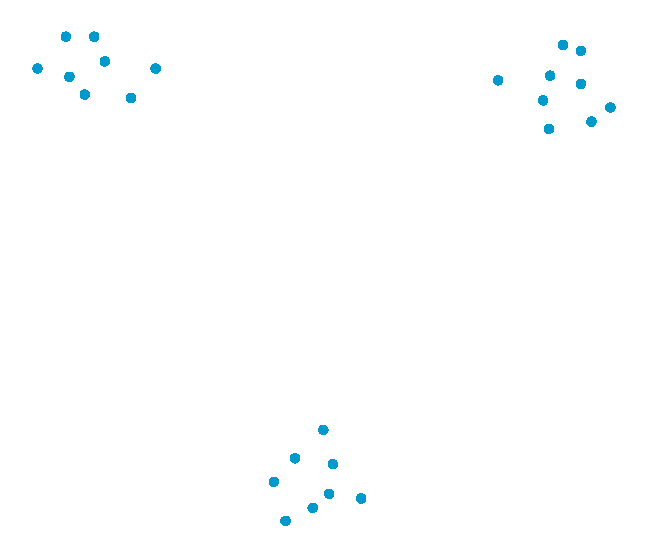
\includegraphics[width=.4\linewidth]{gfx/three_clusters_small.pdf}
    \caption{Dati divisi in più cluster}
    \label{fig:clusters}
  \end{center}
\end{figure}

Ad esempio, consideriamo un insieme di dati come in \cref{fig:clusters}. È chiaro a chi osserva che vi sono tre gruppi di punti, tuttavia la formalizzazione matematica di questa osservazione non è immediata.

Il modo usato dalla TDA è l'\emph{omologia persistente}, di cui diamo un'introduzione informale per poi riprenderlo in (NMDC: inserire riferimento al capitolo). Sia
\begin{equation*}
  X=\{x_1,\dots, x_n\}
\end{equation*}
il nostro insieme di dati. Consideriamo per $\varepsilon>0$ l'insieme
\begin{equation*}
  \widehat{X}_\varepsilon=\bigcup_{0\leq i\leq n} B(x_i,\varepsilon)
\end{equation*}
dove $B(x_i,\varepsilon)$ è la palla di centro $x_i$ e raggio $\varepsilon$. Osserviamo che esiste un intervallo di valori $a \leq \varepsilon \leq b$ per cui $\widehat{X}_\varepsilon$ appare come in \cref{fig:clusters_fat}.

\begin{figure}[h]
  \begin{center}
    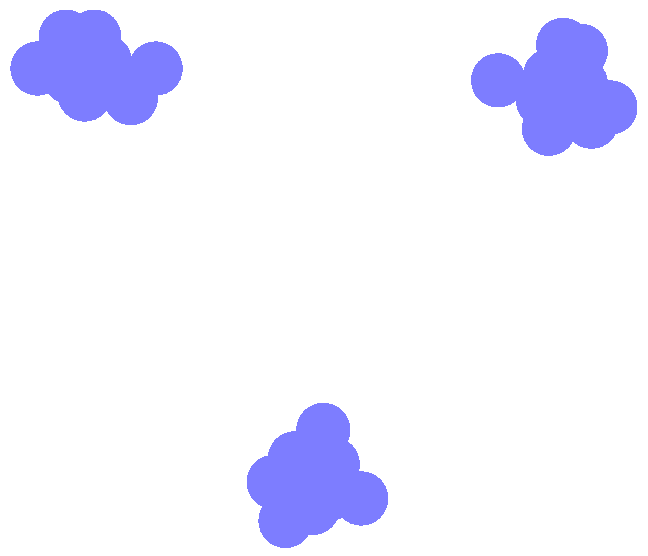
\includegraphics[width=.4\linewidth]{gfx/three_clusters_fat.pdf}
    \caption{$\widehat{X}_\varepsilon$}
    \label{fig:clusters_fat}
  \end{center}
\end{figure}

Allora possiamo possiamo calcolare il numero di componenti connesse di $\widehat{X}_\varepsilon$, o equivalentemente la dimensione del gruppo di omologia $H_{0}(\widehat{X}_\varepsilon;k)$, dove $k$ è un campo. L'osservazione che $X$ è composto essenzialmente da tre componenti è espressa dal fatto che
\begin{equation*}
  \mathrm{dim}_k(H_{0}(\widehat{X}_\varepsilon;k))=3
\end{equation*}
per un intervallo notevole di valori di $\varepsilon$, e da un certo $\overline{\varepsilon}$ in poi diventa~1.

Ovviamente, non è necessario parlare di dimensione del gruppo di omologia $H_{0}$ per discutere del numero di componenti connesse. Tuttavia, se consideriamo l'insieme di dati $X$ come in \cref{fig:circle}, possiamo chiederci come formalizzare l'intuizione che essi sono disposti in forma circolare.

\begin{figure}[h]
  \begin{center}
    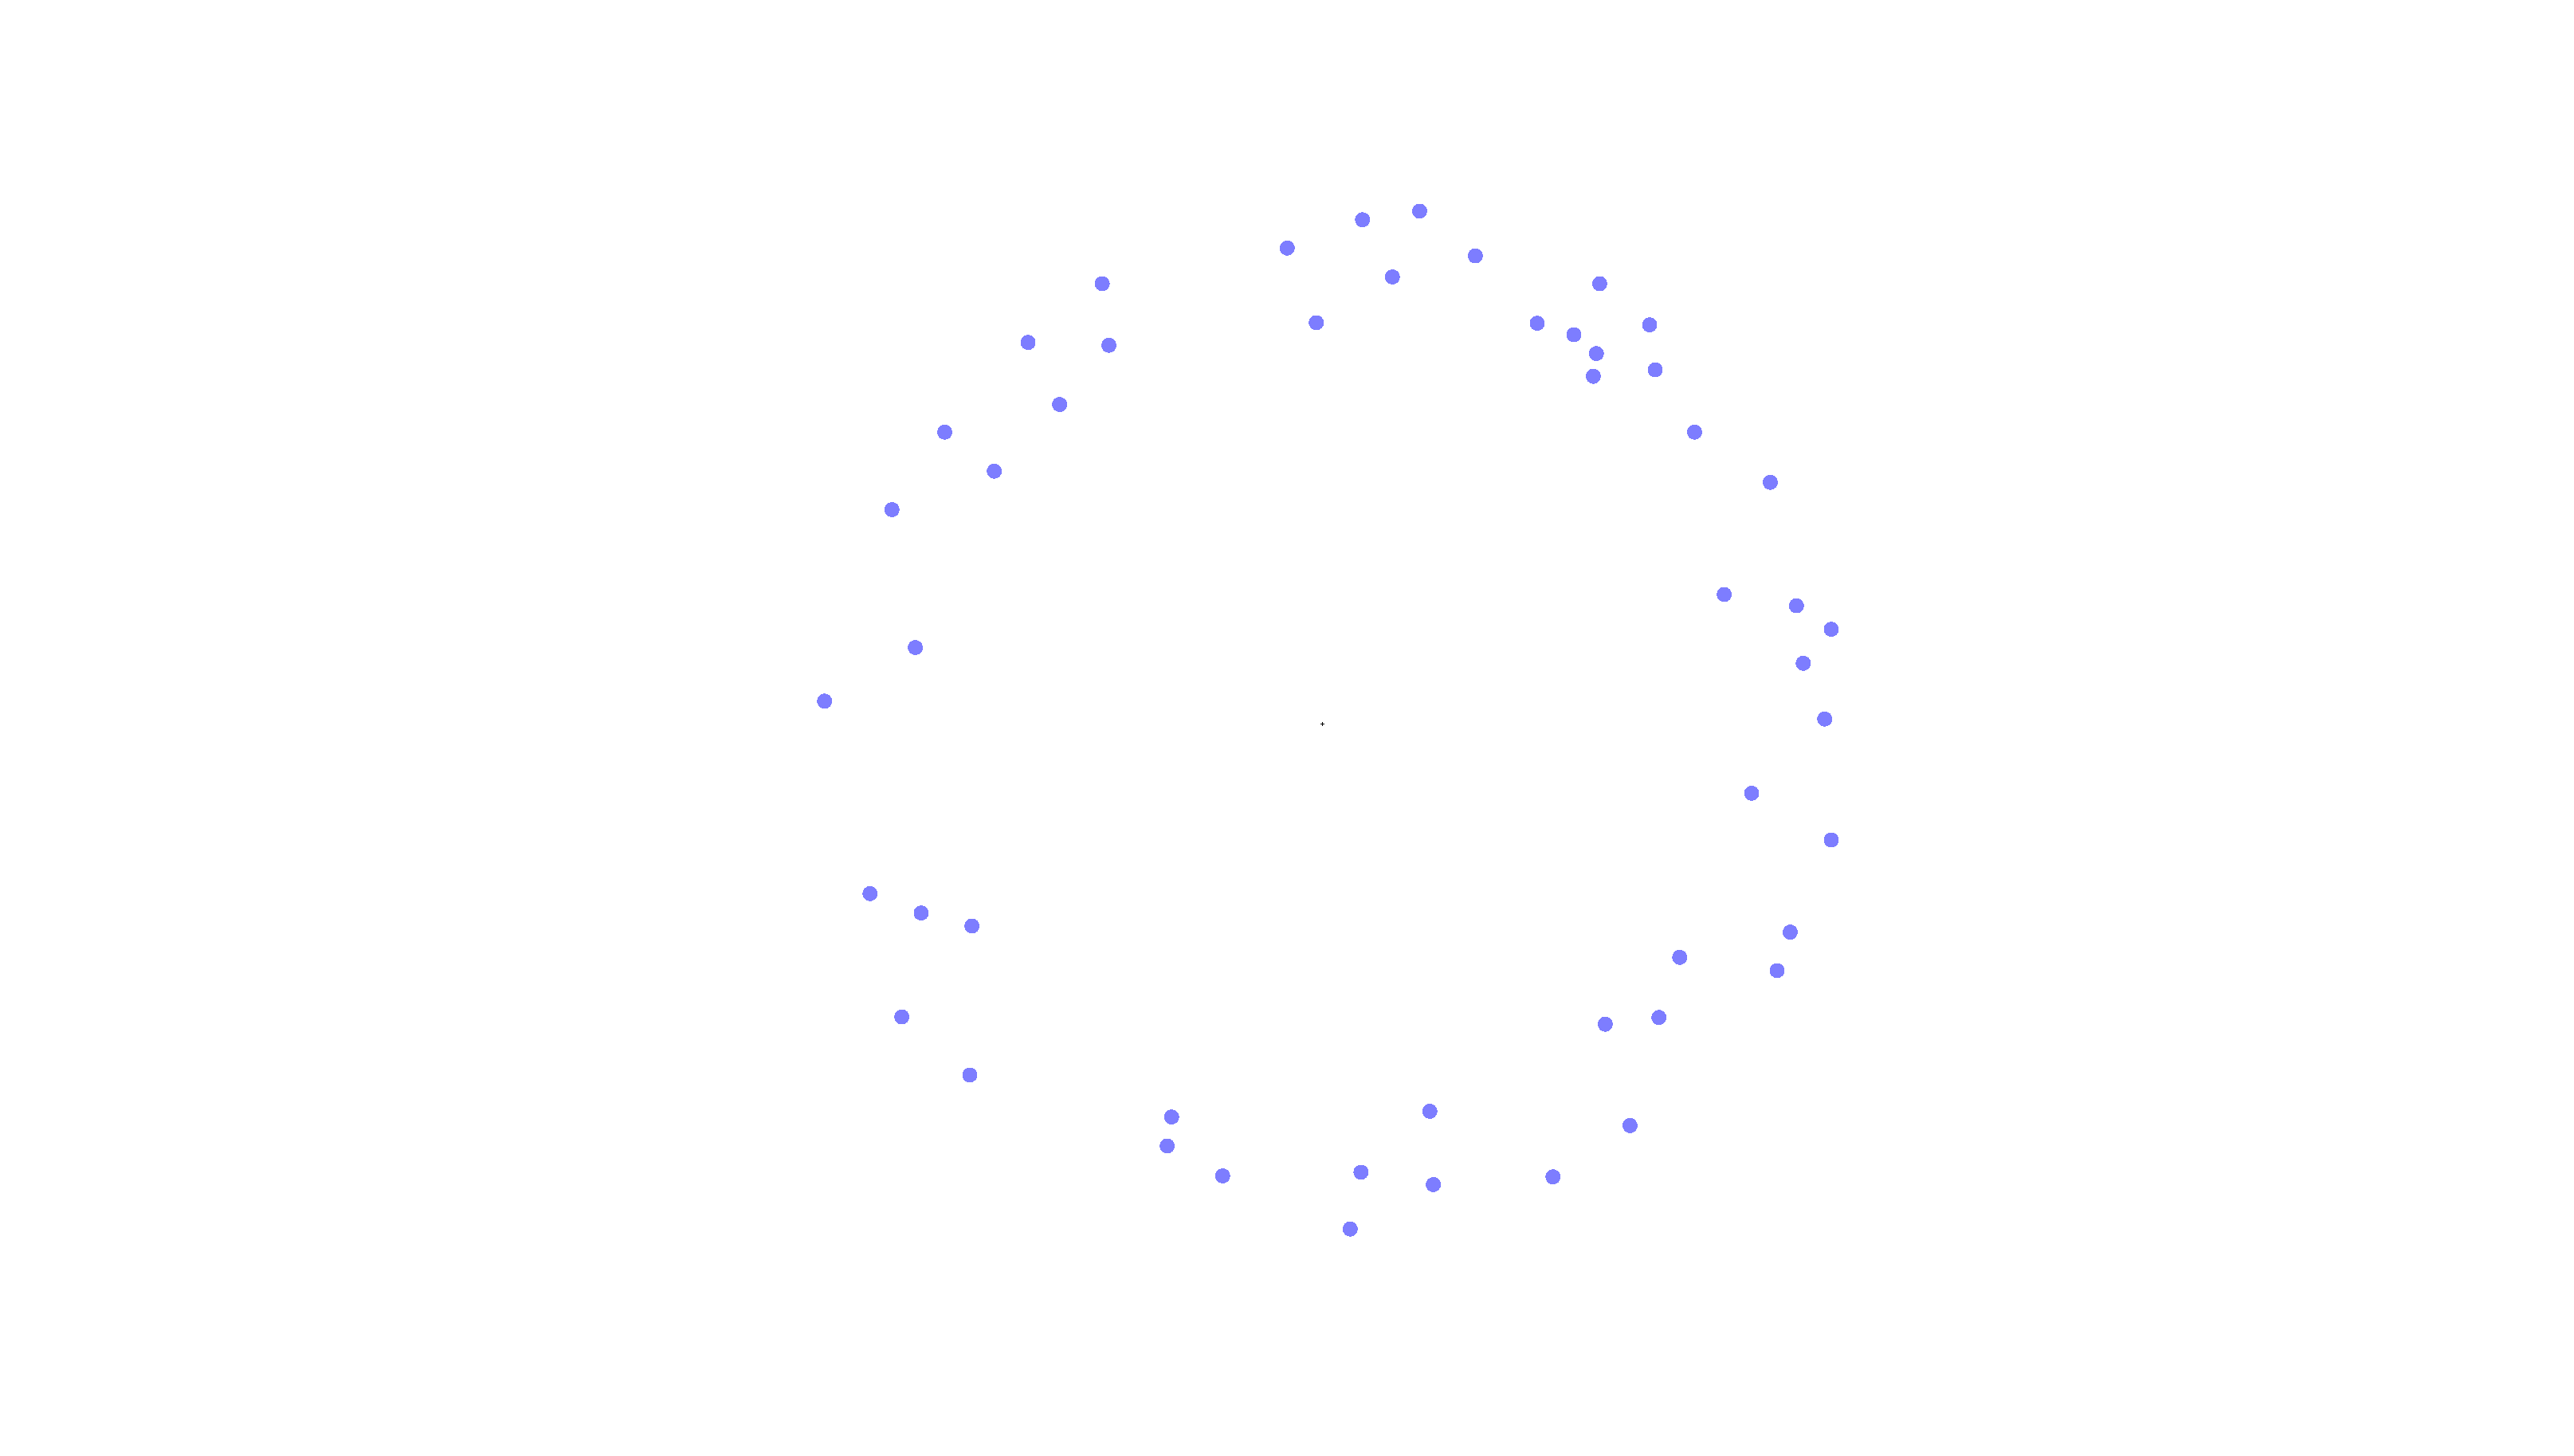
\includegraphics[width=\linewidth]{gfx/statistical_circle.pdf}
    \caption{Campionamento da una corona circolare}
    \label{fig:circle}
  \end{center}
\end{figure}

Ancora una volta possiamo considerare l'insieme $\widehat{X}_\varepsilon$ per diversi valori di $\varepsilon$ come in \cref{fig:circlecomparison} e considerare stavolta il gruppo di omologia $H_{1}(\widehat{X}_\varepsilon;k)$.

\begin{figure}[h]
  \begin{center}
    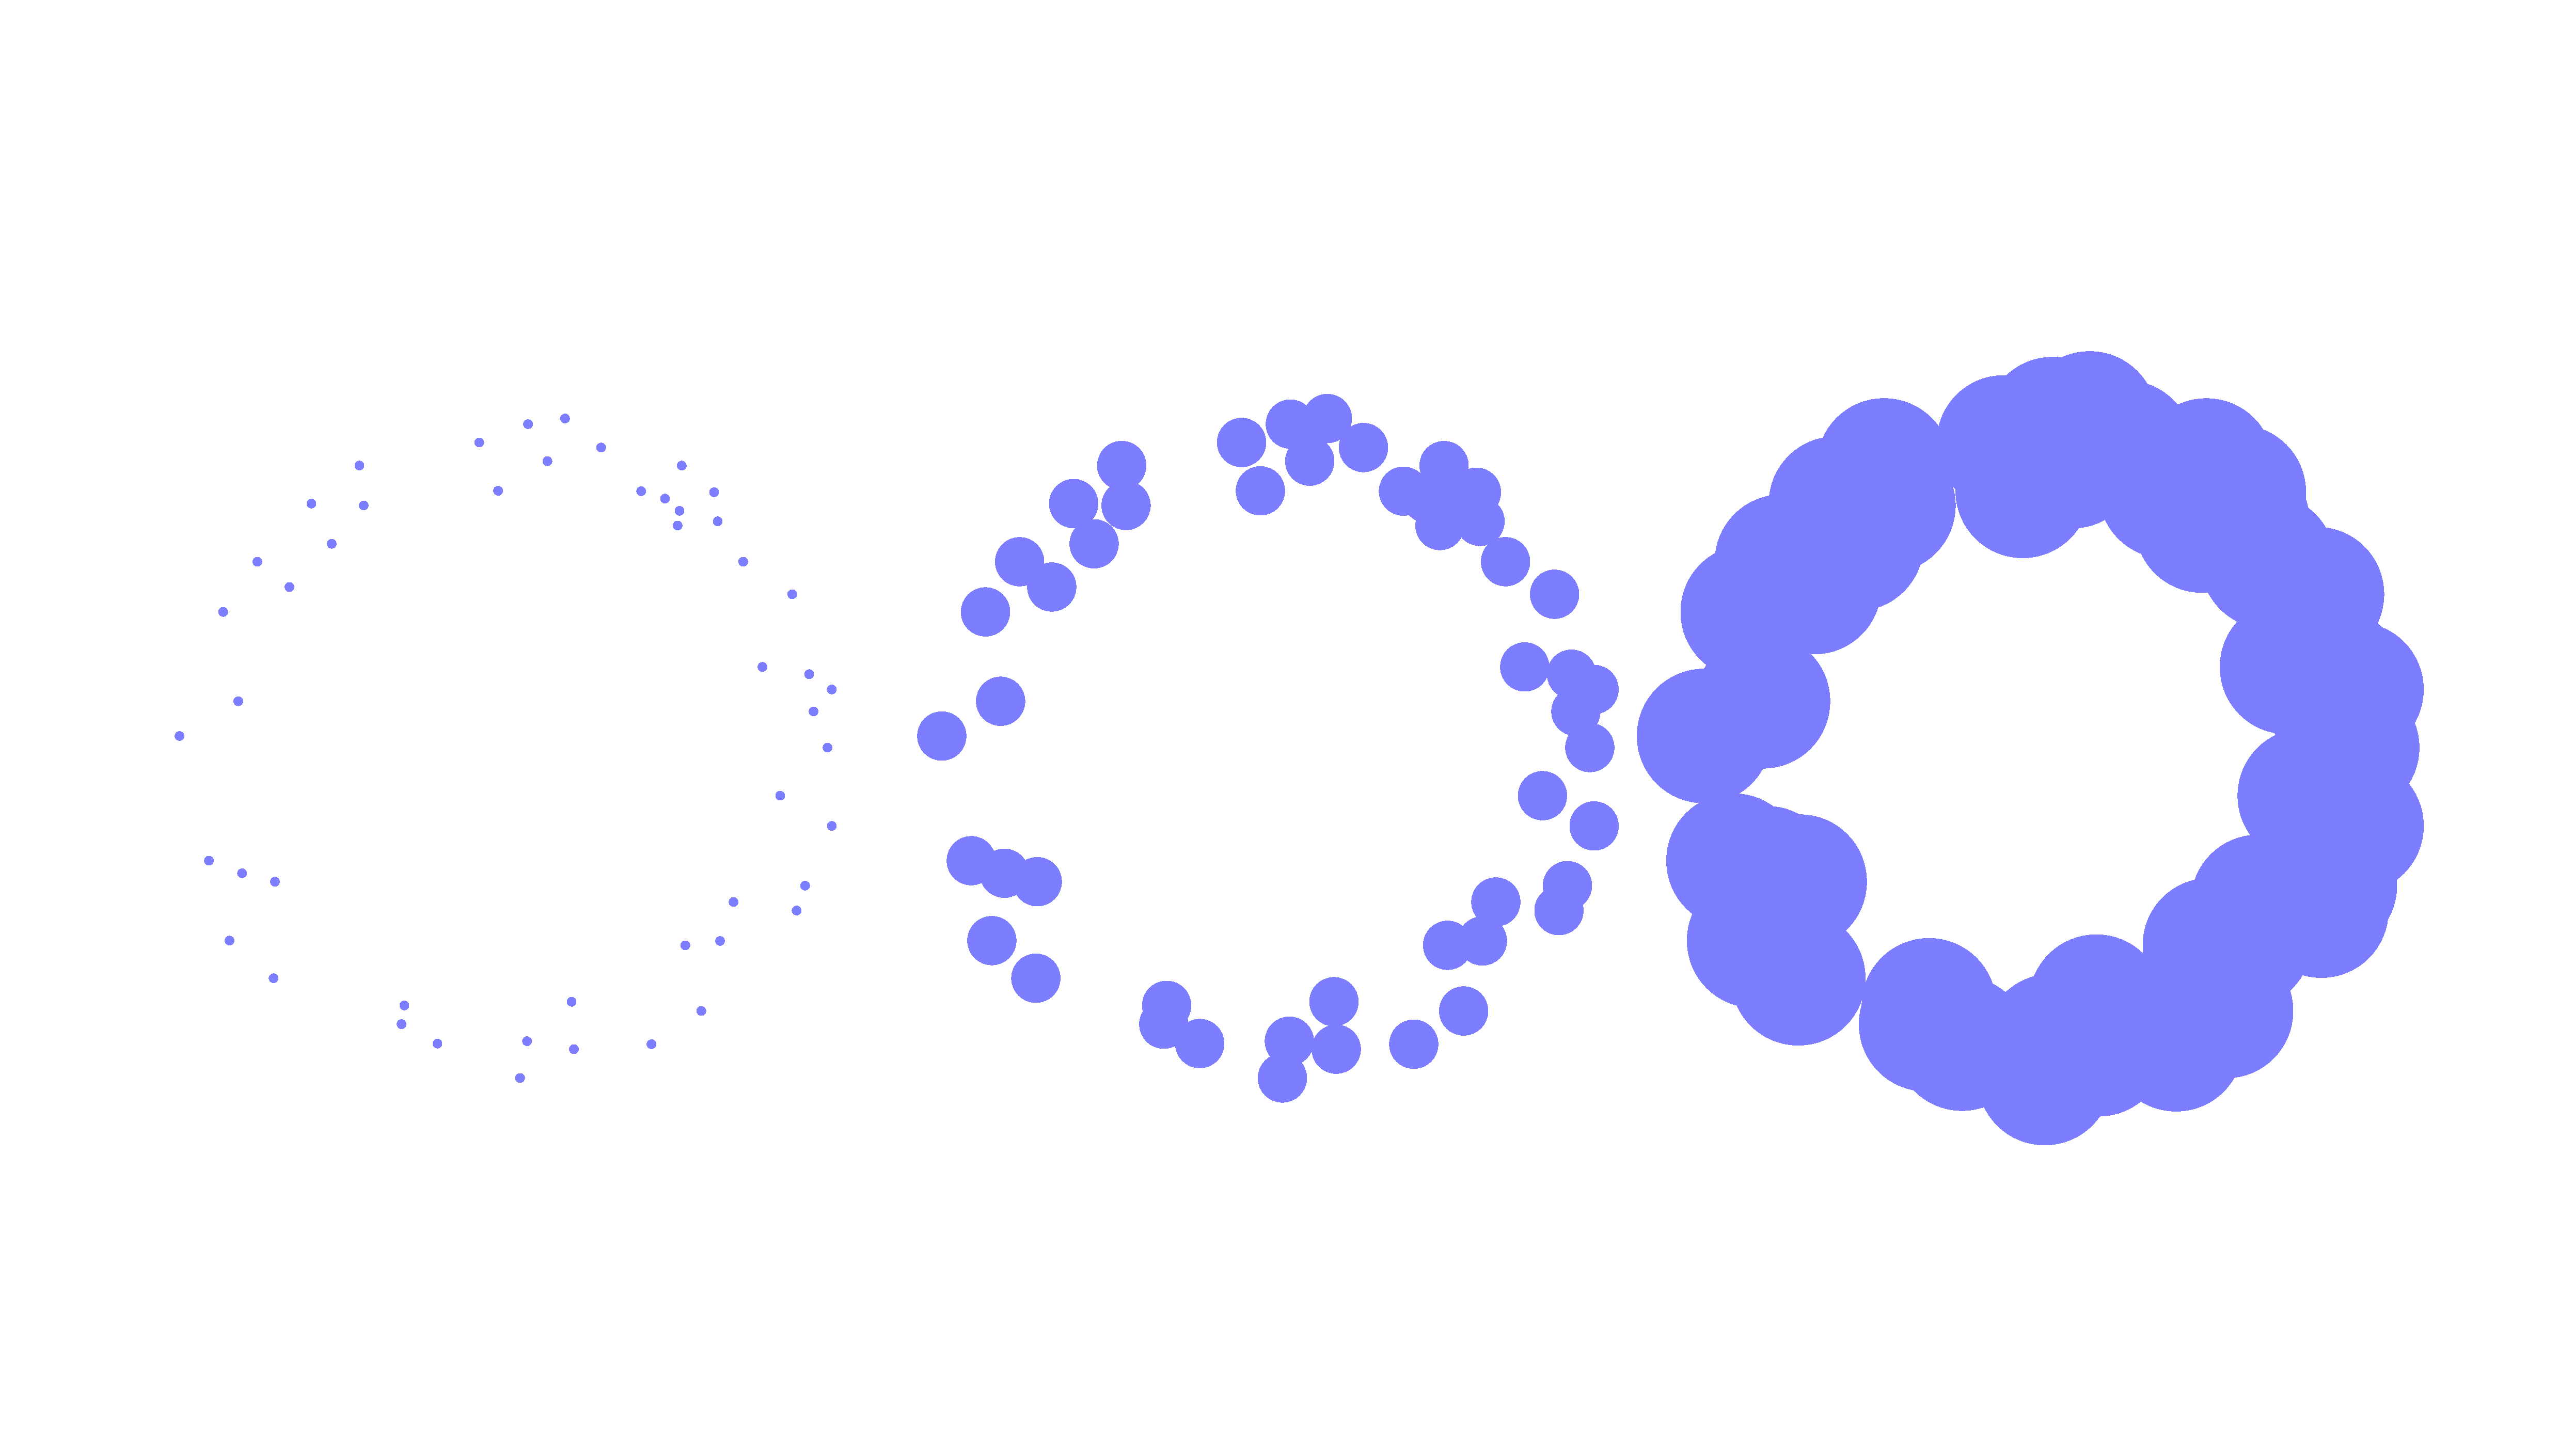
\includegraphics[width=.7\paperwidth]{gfx/statistical_circle_comparison.pdf}
    \caption{$\widehat{X}_\varepsilon$ al variare di $\varepsilon$}
    \label{fig:circlecomparison}
  \end{center}
\end{figure}

La dimensione di $H_1(\widehat{X}_\varepsilon;k)$ varia fino a stabilizzarsi su 1. Questo ci dice che c'è essenzialmente un buco 1-dimensionale nei dati.

Possiamo anche osservare variazioni di struttura al variare della scala di riferimento. Ad esempio, in \cref{fig:moreclusters} possiamo vedere che i tre cluster sulla sinistra collassano in un unico cluster se condiseriamo $\widehat{X}_\varepsilon$ per $\varepsilon \gtrsim e_2/2$.

\begin{figure}[h]
  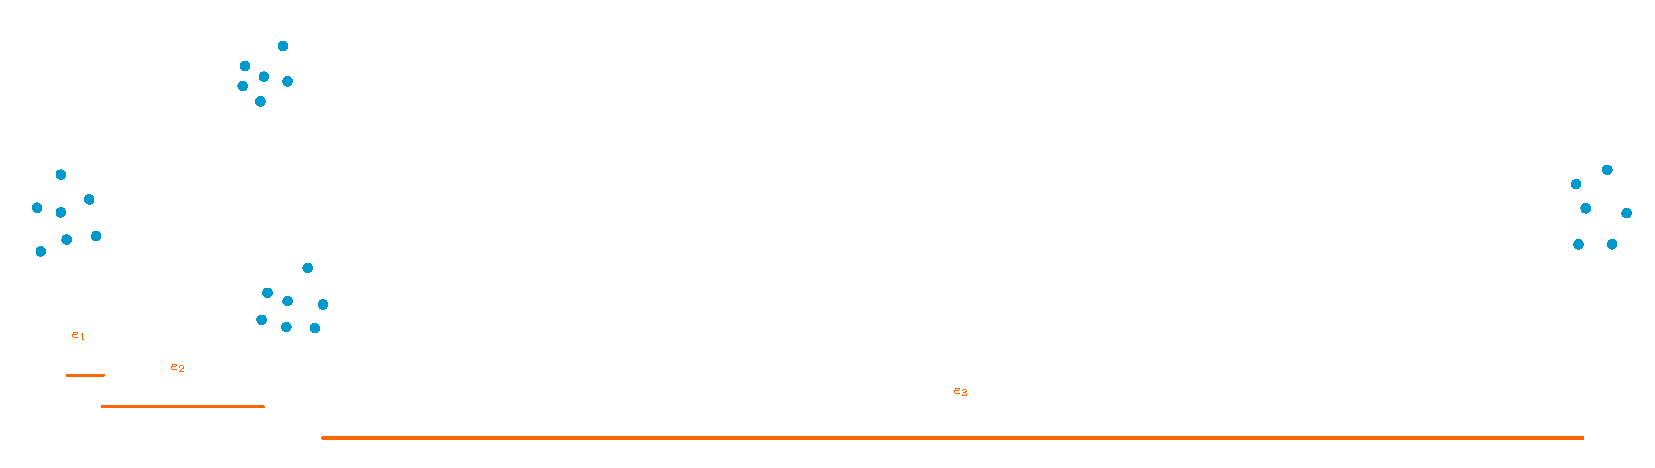
\includegraphics[width=.7\paperwidth]{gfx/more_clusters.pdf}
  \caption{Cluster su scale diverse}
  \label{fig:moreclusters}
\end{figure}

Per visualizzare l'andamento di $dim_k(\widehat{X}_\varepsilon)$ al variare di $\varepsilon$ usiamo un tipo di grafico chiamato \emph{persistence barcode}: per ogni \emph{feature} presente nei dati, disegnamo un segmento orizzontale lungo quanto l'intervallo di lunghezze di $\varepsilon$ in cui la feature persiste, come in \cref{fig:moreclusterbarcode}.

\begin{figure}[h]
  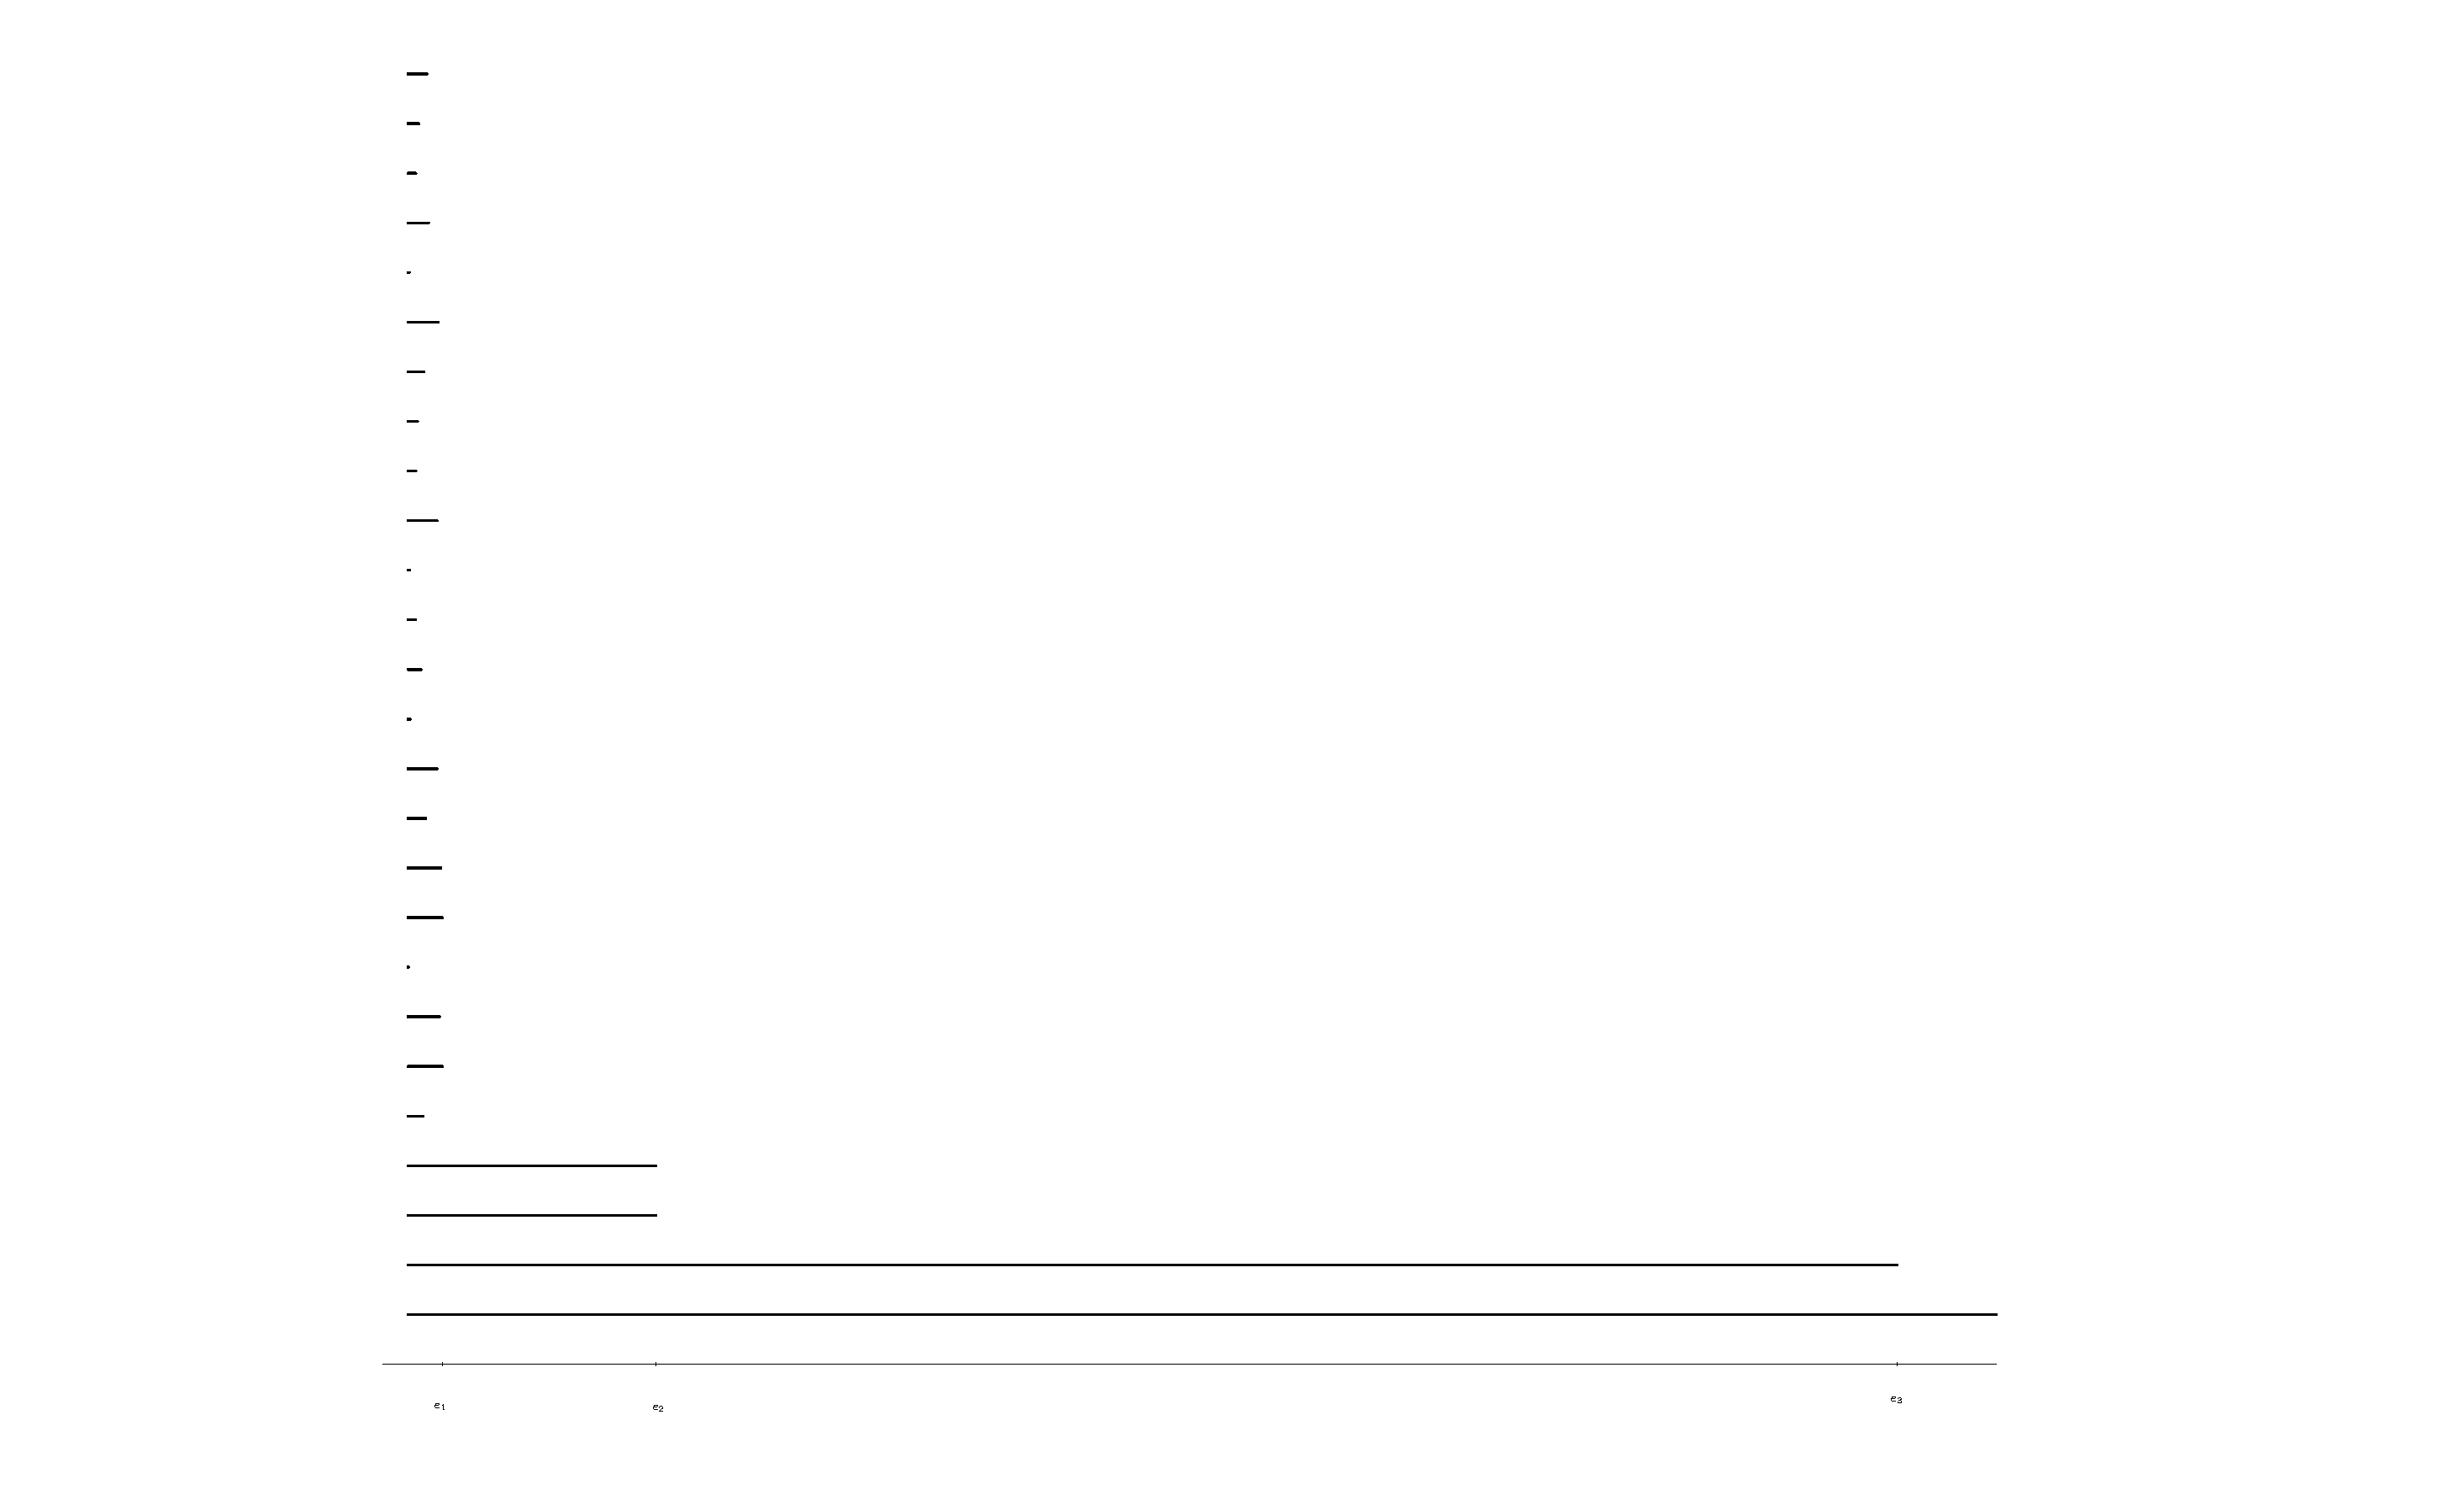
\includegraphics[width=.7\paperwidth]{gfx/more_clusters_barcodes.pdf}
  \caption{Un esempio di persistence barcode}
  \label{fig:moreclusterbarcode}
\end{figure}

Il grafico fa interpretato nel seguente modo: all'inizio vi sono 26 punti distinti, al crescere di $\varepsilon$ questi punti vengono uniti ad altri e quindi il numero si riduce, finché per $\varepsilon \gtrsim e_1/2$ restano essenzialmente 4 cluster, da $e_2/2$ ne restano solo due e da $e_3/2$ il gruppo di omologia $H_0(\widehat{X}_\varepsilon;k)$ diventa banale. (NMDC: aggiusta il grafico del barcode)

Possiamo sempre usare questa rappresentazione grazie alla decomposizione dei persistence barcodes garantita dal teorema (NMDC: aggiungere riferimento).

Un altro aspetto che l'omologia persistente cattura è la relazione fra i gruppi di omologia nelle diverse scale, in particolare $H_*(\widehat{X}_\varepsilon;k)$ è funtoriale rispetto all'ordine di $(\R,\leq)$, cioé se $\varepsilon_1 \leq \varepsilon_2$ allora c'è una mappa $H_*(\widehat{X}_{\varepsilon_1};k)\to H_*(\widehat{X}_{\varepsilon_2};k)$ e se $\varepsilon_1\leq\varepsilon_2\leq\varepsilon_3$, allora la mappa associata a $\varepsilon_1\leq\varepsilon_3$ è uguale alla composizione delle due mappe associate a $\varepsilon_1\leq\varepsilon_2$ e $\varepsilon_2\leq\varepsilon_3$.

Questo ci consente di catturare proprietà come quelle che si osservano in \cref{fig:doublecircle}.

\begin{figure}[ht]
  \begin{center}
    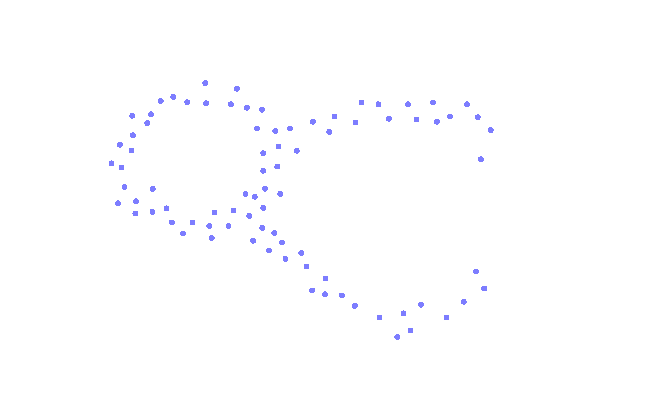
\includegraphics{gfx/double_circle_small.pdf}
    \caption{Un doppio anello}
    \label{fig:doublecircle}
  \end{center}
\end{figure}

In fig. \ref{fig:doublecirclecomparison} osserviamo che al variare di $\varepsilon$ la dimensione di $H_1(\widehat{X}_\varepsilon;k)$ resta 1, tuttavia è chiaro che i due anelli sono due proprietà distinte dei dati. Questa distinzione non è racchiusa nel gruppo di omologia $H_1$, mentre la si vede dal fatto che la mappa
\begin{equation*}
H_1(\widehat{X}_{\varepsilon_1};k)\xto{0}H_1(\widehat{X}_{\varepsilon_2};k)
\end{equation*}
associata a $\varepsilon_1\leq\varepsilon_2$ è il morfismo nullo. Questo ci dice che non ci sono relazioni fra i due gruppi di omologia.

\begin{figure}[ht]
  \begin{center}
    \begin{subfigure}[b]{.4\textwidth}
      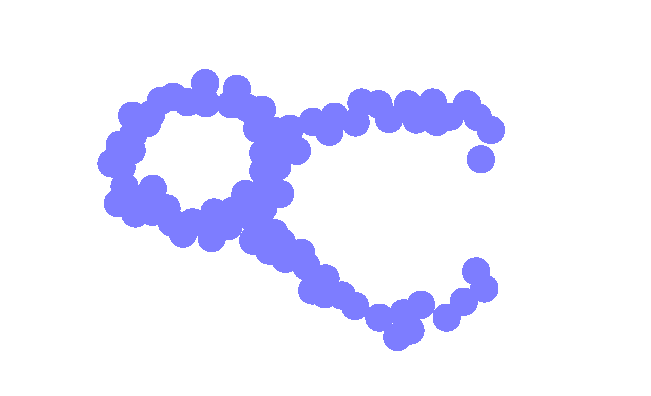
\includegraphics[width=\textwidth]{gfx/double_circle_medium.pdf}
      \caption{$\widehat{X}_{\varepsilon_1}$}
    \end{subfigure}
    \begin{subfigure}[b]{.4\textwidth}
      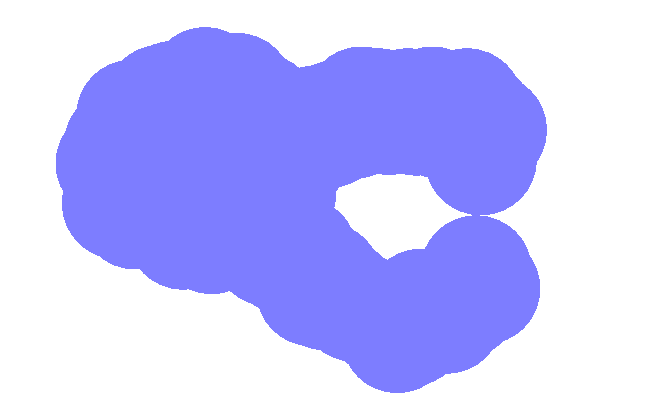
\includegraphics[width=\textwidth]{gfx/double_circle_fat.pdf}
      \caption{$\widehat{X}_{\varepsilon_2}$}
    \end{subfigure}
    \caption{Variazione delle proprietà di $\widehat{X}_\varepsilon$}
  \end{center}
  \label{fig:doublecirclecomparison}
\end{figure}

(NMDC:dire qualcosa sull'algoritmo Mapper?)

Nel resto del capitolo ci occuperemo di costruire l'omologia persistente, con attenzione all'aspetto computazionale.

\clearpage

\section{Omologia simpliciale}

\begin{sloppypar}
  Fissato un campo $k$, ad ogni spazio topologico possiamo associare una successione di $k$-spazi vettoriali $H_i(X;k)$ detti \emph{gruppi di omologia}. Per la precisione si tratta di un $\partial$-funtore (co)omologico ${H_*(-;k):\Top \to \Vectk}$. Nel resto della sezione ci occuperemo di definire in modo operativo questi gruppi.
\end{sloppypar}

Esistono diversi modi di calcolare i gruppi di omologia. Il più generale e potente è quello di utilizzare l'omologia singolare, tuttavia questa risulta scomoda da usare in pratica perché richiede di lavorare con quozienti di spazi vettoriali di dimensione più che numerabile. Per aggirare il problema definiremo soltanto l'omologia simpliciale.

In virtù degli assiomi di Eilenberg-Steenrod \cite{Eilenberg1945, Eilenberg} le due definizioni sono equivalenti (almeno per gli spazi che andremo a considerare). Per una trattazione più dettagliata si vedano \cite{Hatcher2015} o \cite{Rotman1988}.

Gli spazi $\widehat{X}_\varepsilon$, usati nell'introduzione, sono comodi per introdurre un'idea intuitiva di persistenza, tuttavia non sono l'ambiente naturale in cui lavorare, quindi non verranno più usati nella trattazione formale. Si osservi, però, che l'omologia di $\widehat{X}_\varepsilon$ è equivalente all'omologia del complesso di \v{C}ech di parametro $\varepsilon$ associato a $X$. Per questioni di comodità, tuttavia, noi lavoreremo principalmente con il complesso di Vietoris-Rips.
